\section{Tracking}

The tracking task has been performed exclusively on the grid topology because, in general, it produces better results.
We have analyzed two different cases: in the first one (Figure \ref{fig: target moving along the diagonal}) the target 
is moving along the diagonal of the room, while in the second one (Figures \ref{fig: target moving randomly 1e2} and \ref{fig: target moving randomly 5e2}), the target 
is changing it's position randomly at every single step.

\begin{figure}[H]
    \begin{subfigure}{0.45\textwidth}
        \centering
        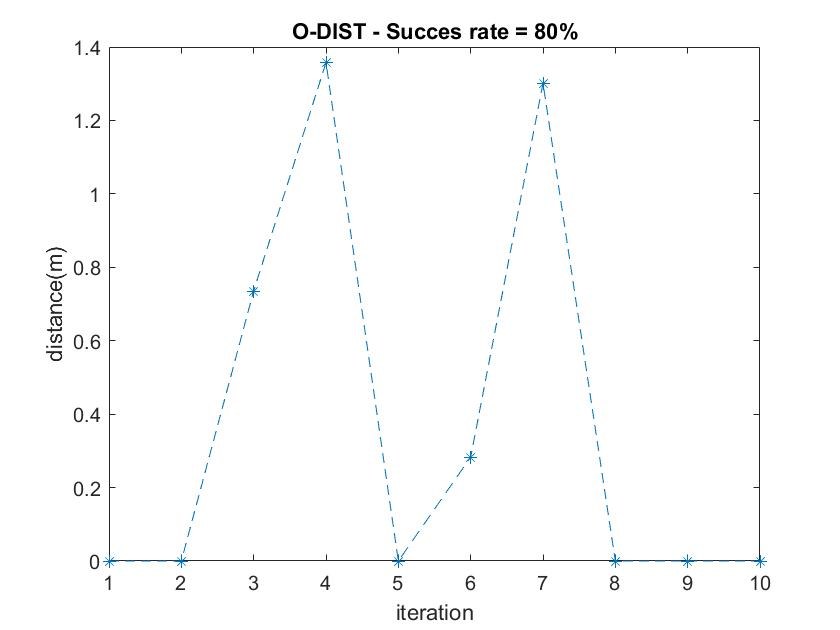
\includegraphics[width=\textwidth]{img/O-DIST_diagonal_distance.jpg}
        \caption{Success rate of 80\%}
    \end{subfigure}
    \hfill
    \begin{subfigure}{0.45\textwidth}
        \centering
        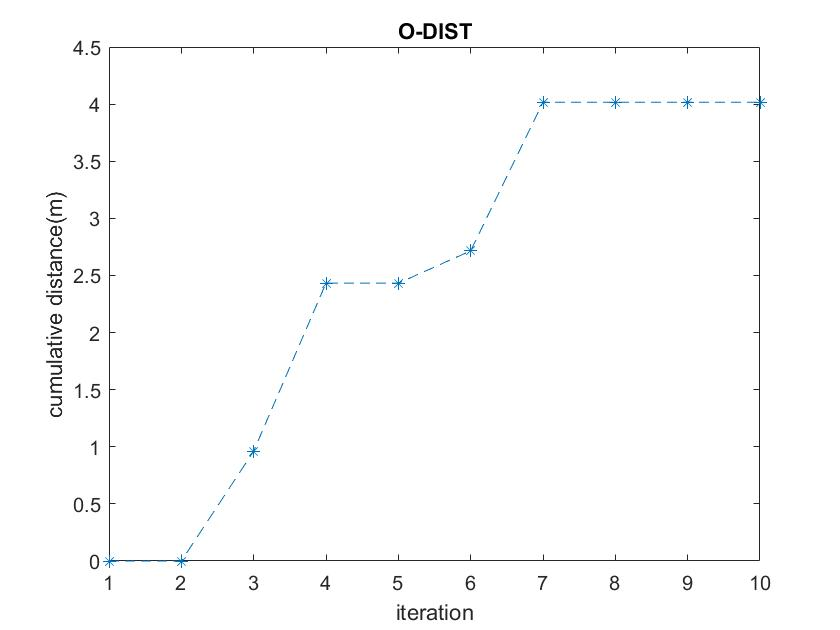
\includegraphics[width=\textwidth]{img/O-DIST_diagonal_cumdist.jpg}
        \caption{Cumulative distance}
    \end{subfigure}
    \caption{O-DIST algorithm performed on uniform topology with the target moving along the diagonal of the room ($\epsilon=10^{-6},\,T=10^2$)}
    \label{fig: target moving along the diagonal}
\end{figure}

\begin{figure}[H]
    \begin{subfigure}{0.45\textwidth}
        \centering
        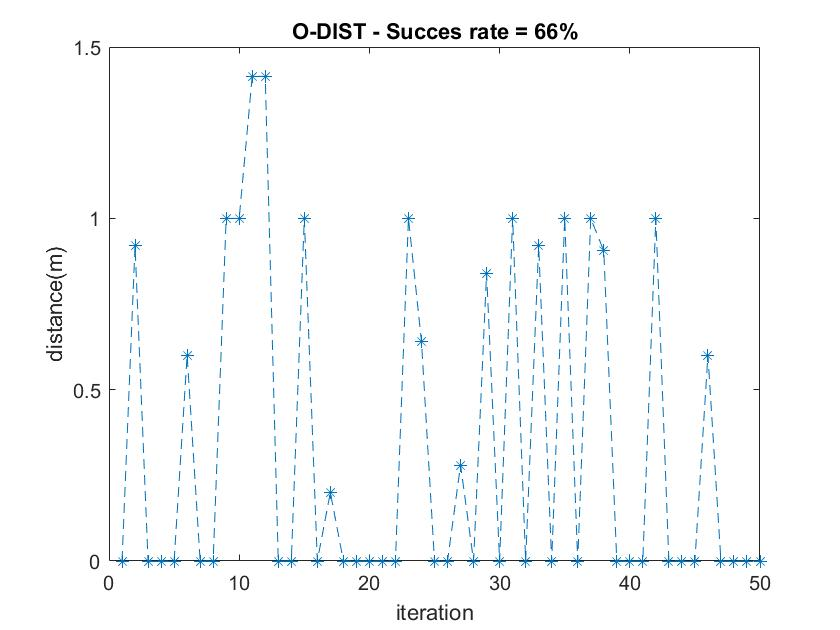
\includegraphics[width=\textwidth]{img/O-DIST_casual_distance_1e2.jpg}
        \caption{Success rate of 66\%}
    \end{subfigure}
    \hfill
    \begin{subfigure}{0.45\textwidth}
        \centering
        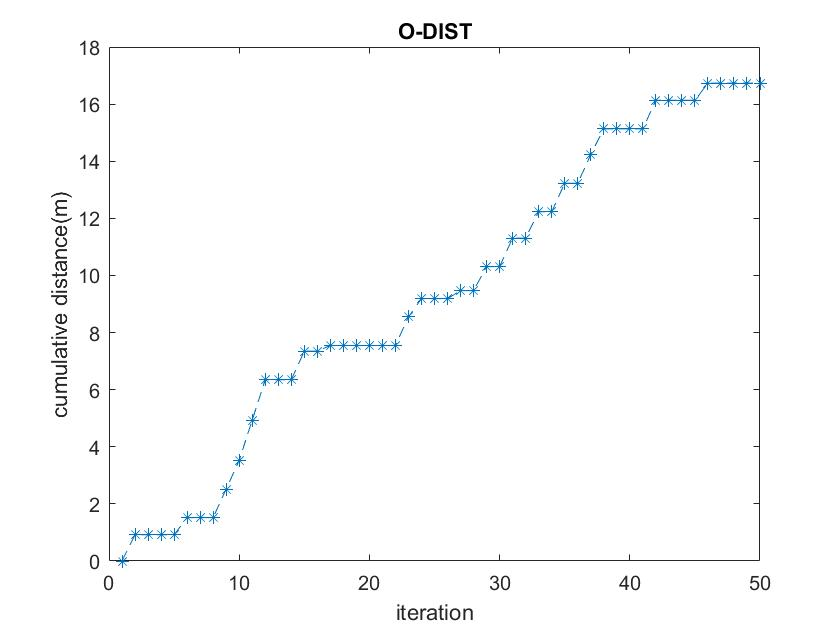
\includegraphics[width=\textwidth]{img/O-DIST_casual_cumdist_1e2.jpg}
        \caption{Cumulative distance}
    \end{subfigure}
    \caption{O-DIST algorithm performed on uniform topology with the target moving randomly in the room ($\epsilon=10^{-6},\,T=5\cdot10^2$)}
    \label{fig: target moving randomly 1e2}
\end{figure}

With $10^2$ maximum number of iterations, the algorithm is not precise, in fact the convergence is not achieved. However, 
the wrong estimated cell is always the adjacent to the correct one.\par 
To improve the accuracy, we can increase the maximum number of iterations from $10^2$ to $5\cdot10^2$. As we can see in 
Figure \ref{fig: target moving randomly 5e2}, we obtained better results in terms of success rate (from $66\%$ to $86\%$) 
and cumulative distance.

\begin{figure}[H]
    \begin{subfigure}{0.45\textwidth}
        \centering
        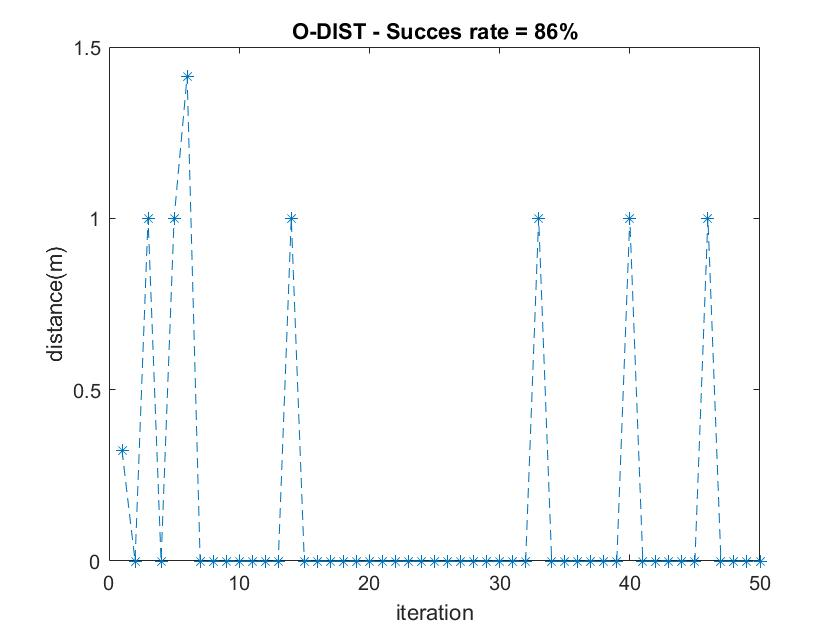
\includegraphics[width=\textwidth]{img/O-DIST_casual_distance_5e2.jpg}
        \caption{Success rate of 66\%}
    \end{subfigure}
    \hfill
    \begin{subfigure}{0.45\textwidth}
        \centering
        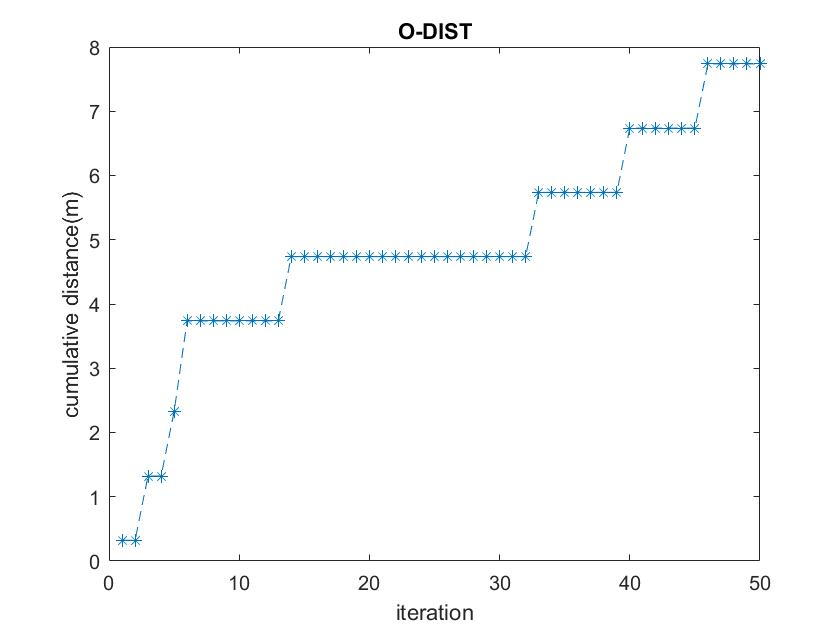
\includegraphics[width=\textwidth]{img/O-DIST_casual_cumdist_5e2.jpg}
        \caption{Cumulative distance}
    \end{subfigure}
    \caption{O-DIST algorithm performed on uniform topology with the target moving randomly in the room ($\epsilon=10^{-6},\,T=5\cdot10^{2}$)}
    \label{fig: target moving randomly 5e2}
\end{figure}